\chapter{Especificación de requisitos}\label{cap:especificacion_requisitos}

\section{Introducción}

Este capítulo se dedica a la especificación detallada de los requisitos del sistema, abarcando tanto los requisitos \textit{funcionales} como los \textit{no funcionales}, así como los requisitos de \textit{información} y de \textit{interfaz}. Antes de entrar en los detalles específicos de estos requisitos, se proporciona una descripción funcional del simulador, resaltando los módulos identificados previamente. Posteriormente, se identificarán los actores que interactuarán con la aplicación.

\section{Actores} \label{sec:actores-req}

El software diseñado en este proyecto está destinado a un entorno educativo, dirigido principalmente a \textit{profesores} y \textit{estudiantes}. A pesar de esta diferenciación en los roles, la aplicación no distinguirá funcionalmente entre estos usuarios, ya que ambos tendrán acceso a las mismas funcionalidades. Por lo tanto, cualquier referencia a los \textit{actores} de la aplicación se aplicará de manera uniforme a todos los usuarios finales, independientemente de su rol específico.


\section{Descripción modular del sistema}

El sistema se compone de varios módulos integrados, cada uno con un propósito específico. A continuación, se describen en detalle los módulos principales que conforman la aplicación:

\begin{itemize}
\item Editor de gramáticas.
\item Simulador gráfico descendente.
\item Tutorial.
\item Sistema de ayuda.
\end{itemize}

 La Figura \ref{fig:diagrama-descomposicion} muestra la descomposición modular del sistema.
 
\begin{figure}[!ht]
   \begin{center} 
     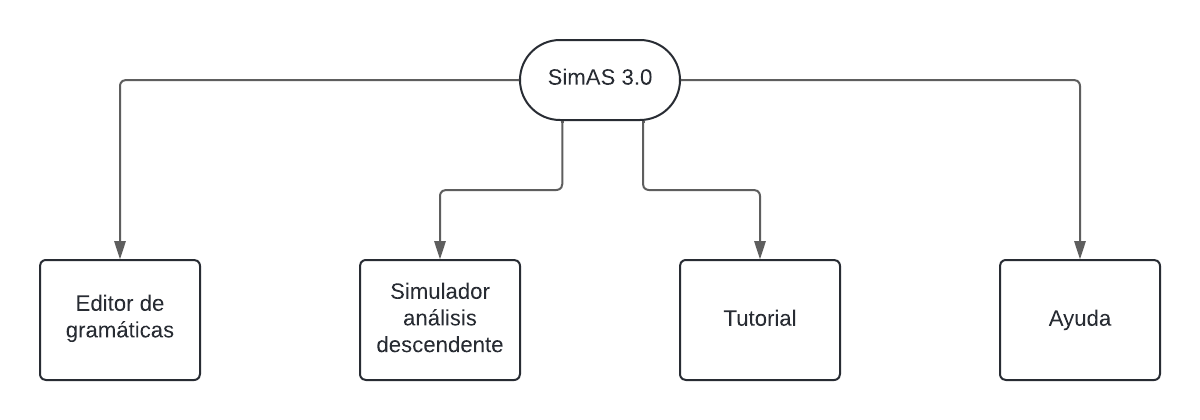
\includegraphics[width=1\textwidth]{figuras/Cap6/diagrama-descomposicion.png}
     \caption{Descomposición modular del sistema}\label{fig:diagrama-descomposicion}
   \end{center}
 \end{figure}


\subsection{Módulo del Editor de Gramáticas}

El editor de gramáticas es una herramienta fundamental dentro del sistema, permitiendo a los usuarios crear y modificar gramáticas de contexto libre. Las funcionalidades específicas de este módulo incluyen:

\begin{enumerate}
    \item \textbf{Creación de gramáticas}: los usuarios pueden definir nuevas gramáticas, especificando sus componentes esenciales, como símbolos terminales, no terminales, el símbolo inicial y las reglas gramaticales.
    \item \textbf{Gestión de vocabulario}: permite a los usuarios añadir y eliminar símbolos del vocabulario de una gramática, gestionando tanto los símbolos terminales como los no terminales, que son necesarios para formar las reglas.
    \item \textbf{Gestión de reglas gramaticales o producciones}: facilita la introducción, modificación y eliminación de las reglas gramaticales de una gramática, asegurando que no haya duplicados.
    \item \textbf{Validación de gramáticas}: este proceso asegura que la gramática es válida, verificando que todos los símbolos sean accesibles y generadores:
    \begin{itemize}
        \item \textbf{Accesibilidad}: un símbolo se considera accesible si se puede alcanzar desde el símbolo inicial mediante una serie de derivaciones.
        \item \textbf{Generatividad}: un símbolo es generativo si puede derivar en una cadena de símbolos terminales o la cadena vacía.
    \end{itemize}
    
    En caso de errores, se informará al usuario y se proporcionarán sugerencias para la corrección.
    \item \textbf{Almacenamiento de gramáticas}: los usuarios pueden guardar sus gramáticas en archivos para uso futuro, independientemente de si la gramática ha sido completamente validada.
    \item \textbf{Carga de gramáticas}: permite cargar gramáticas desde archivos existentes, validando que no estén corruptos y notificando al usuario  cualquier error durante el proceso.
    \item \textbf{Consulta de gramáticas}: muestra la estructura completa de la gramática actual, incluyendo todos sus componentes, y permite generar un informe detallado.
\end{enumerate}

\subsection{Módulo del Simulador Gráfico Descendente Predictivo}

Este módulo constituye el núcleo de la aplicación, proporcionando la capacidad de simular el análisis sintáctico descendente predictivo de manera visual e interactiva. A continuación se detalla su funcionamiento.

\subsubsection{Creación y carga de gramáticas}

El primer paso en el proceso de simulación es la creación o carga de una gramática. Los usuarios pueden utilizar el módulo de edición de gramáticas para definir una nueva gramática o cargar una existente desde un archivo. Es fundamental que la gramática haya sido validada previamente para asegurar su correcta estructura y funcionalidad antes de ser utilizada en la simulación.

\subsubsection{Generación de conjuntos \textit{Primero} y \textit{Siguiente}}

Una vez que la gramática está lista, se procede a la generación de los conjuntos Primero y Siguiente. Estos conjuntos son esenciales para la construcción de la tabla predictiva, ya que determinan las posibles reglas gramaticales o producciones que pueden aplicarse durante el análisis de una cadena de entrada.

\subsubsection{Construcción de la tabla predictiva}

Después de obtener los conjuntos Primero y Siguiente, se debe construir la tabla predictiva del análisis sintáctico descendente. Esta tabla es una guía que indica qué regla gramatical debe aplicarse para cada combinación de símbolo de entrada y símbolo no terminal. La tabla predictiva es fundamental para la correcta derivación de la cadena de entrada y facilita la detección y manejo de errores durante el análisis.

\subsubsection{Implementación de funciones de recuperación de errores}

Aunque esta parte es opcional, la implementación de funciones de recuperación de errores es altamente recomendable. Estas funciones se utilizan para manejar las celdas vacías en la tabla predictiva, proporcionando mecanismos para continuar el análisis sintáctico en caso de encontrar un error. Entre las funciones de recuperación de errores se incluyen:

\begin{itemize}
  \item Eliminar el símbolo actual de la entrada.
  \item Insertar un nuevo símbolo terminal en la entrada, con funciones específicas para cada símbolo terminal.
  \item Terminar el análisis si hay un final inesperado de la entrada.
\end{itemize}

\subsubsection{Simulación del análisis sintáctico descendente  predictivo}

Con la tabla predictiva completada, el usuario puede introducir una cadena de entrada para simular el análisis sintáctico descendente predictivo. Durante esta fase, el simulador utilizará la tabla predictiva para derivar la cadena de entrada, gestionando los errores según las funciones de recuperación definidas. El sistema informará al usuario sobre el estado de la cadena de entrada, indicando si es reconocida o si se han producido errores. La aplicación permitirá mostrar la derivación de la cadena de entrada generada por el análisis sintáctico descendente predictivo.

\subsubsection{Generación del árbol sintáctico descendente}

Una característica avanzada del simulador es la capacidad de generar el árbol sintáctico descendente. Esta opción permite a los usuarios visualizar la estructura jerárquica de la derivación de la cadena de entrada en tiempo real, mejorando su comprensión del proceso de análisis sintáctico. El árbol sintáctico se construye de forma paralela a la simulación, proporcionando una representación gráfica de cada paso del análisis.

\subsubsection{Creación de informes}

Finalmente, tras la simulación, se generará un informe detallado que documenta todo el proceso. Este informe, disponible en formatos PDF o HTML, incluirá:

\begin{itemize}
  \item Información detallada sobre la gramática utilizada.
  \item Los conjuntos Primero y Siguiente generados.
  \item La tabla predictiva construida.
  \item Las funciones de recuperación de errores definidas.
  \item La cadena de entrada y su estado (reconocida o no).
  \item Los errores detectados durante el análisis y cómo fueron manejados.
  \item La derivación de la cadena de entrada generada por el análisis sintáctico descendente predictivo.
  \item El árbol sintáctico asociado a la derivación de la cadena de entrada generada por el análisis sintáctico descendente predictivo.
\end{itemize}

Este informe puede ser almacenado en disco por el usuario, proporcionando una referencia completa y detallada del análisis sintáctico descendente realizado.


\subsection{Módulo del Tutorial}

Este módulo tiene un enfoque educativo, diseñado para proporcionar todos los objetivos pedagógicos del proyecto. Se ubicará de manera accesible desde cualquier otro módulo del programa, permitiendo al usuario consultarlo en cualquier momento, incluso mientras interactúa con otras partes de la aplicación.

\subsubsection{Estructura del tutorial}

El tutorial se organizará en las siguientes secciones:

\begin{enumerate}
    \item \textbf{Introducción y fundamentos teóricos:} esta sección cubre los conceptos teóricos fundamentales del análisis sintáctico, con un enfoque en las gramáticas de contexto libre. Proporcionará una base sólida para entender los principios detrás del análisis sintáctico descendente.

    \item \textbf{Lecciones de análisis sintáctico descendente:} aquí se explicarán los métodos de análisis sintáctico descendente predictivo. Las lecciones estarán estructuradas de manera que el usuario pueda seguir cada paso del proceso de análisis de manera clara y comprensible.

    \item \textbf{Ejemplos y ejercicios prácticos:} esta parte del tutorial incluirá una serie de ejercicios prácticos y ejemplos resueltos. Los usuarios podrán realizar estos ejercicios y verificar sus respuestas utilizando el simulador. Esta sección está diseñada para reforzar el aprendizaje a través de la práctica y la aplicación de conceptos teóricos.
\end{enumerate}

\subsection{Módulo de Ayuda}

El módulo de \textit{Ayuda} proporciona una guía completa sobre el uso de la aplicación. Está diseñado para ser una referencia detallada que abarca todos los aspectos del funcionamiento del programa.

\subsubsection{Contenidos de la ayuda}

\begin{enumerate}
    \item \textbf{Introducción a la aplicación:}
    esta sección presentará una visión general de la aplicación, describiendo sus objetivos y las principales funcionalidades que ofrece. Proporcionará una primera impresión de lo que los usuarios pueden esperar del programa.

    \item \textbf{Requisitos de instalación y procedimiento:}
    aquí se detallarán los requisitos del sistema necesarios para ejecutar la aplicación, así como las instrucciones paso a paso para su instalación y desinstalación. Se incluirán también soluciones a posibles problemas que puedan surgir durante estos procesos.

    \item \textbf{Guía de la interfaz de usuario:}
    esta sección ofrecerá una explicación detallada de los diferentes componentes de la interfaz del simulador. Se proporcionarán descripciones de cada elemento de la interfaz y su funcionalidad, ayudando a los usuarios a navegar y utilizar el programa de manera eficiente.

    \item \textbf{Descripción de los módulos del programa:}
    En esta parte, se explicará en profundidad el funcionamiento de cada uno de los módulos de la aplicación. Se incluirán instrucciones específicas sobre cómo utilizar cada módulo, junto con ejemplos prácticos y consejos para maximizar su uso.
\end{enumerate}


 \section{Requisitos funcionales}

En esta sección se recogen los requisitos funcionales de la aplicación, los cuales se denotarán como \textbf{RF-$<$acrónimo del módulo$>$-$<$número de requisito$>$}. Los requisitos funcionales se encuentran agrupados según los módulos funcionales del Sistema, que son las siguientes:

\begin{itemize}
 \item \textbf{Editor de gramáticas}: requisitos funcionales del \textit{editor de gramáticas}.
 \item \textbf{Simulador}: requisitos funcionales del \textit{simulador}.
 \item \textbf{Tutorial}: requisitos funcionales del \textit{tutorial}.
 \item \textbf{Ayuda}: requisitos funcionales  del \textit{ayuda}.
\end{itemize}


\subsection{Requisitos funcionales del Editor de gramáticas}\label{sec:requisitos-funcionales-editor}

Esta sección detalla todos los requisitos funcionales del \textit{Editor de gramáticas}, listados a continuación:

\begin{itemize}
    \item \textbf{RF-E-1}. El editor de gramáticas permitirá al usuario crea una nueva gramática de contexto libre. 
    \item \textbf{RF-E-2}. El editor permitirá la creación y modificación del conjunto de símbolos de la gramática (símbolos terminales y no terminales):
    \begin{itemize}
      \item \textbf{RF-E-2.1}. También admitirá el uso de caracteres especiales, tales como $\epsilon$ y $\rightarrow$, entre otros.
    \item \textbf{RF-E-2.2}. Será posible definir símbolos personalizados para la construcción de reglas, como, por ejemplo, $<$asignación$>$.
    \item  \textbf{RF-E-2.3}. Se gestionarán y notificarán todos los errores relacionados con la creación y edición de símbolos de manera clara y concisa para el usuario.
    \item \textbf{RF-E-2.4}. Las reglas de la gramática se ordenarán en función del símbolo no terminal de su parte izquierda.
    \end{itemize}
    
\item \textbf{RF-E-3}. El editor permitirá crear reglas gramaticales utilizando los símbolos definidos por el usuario. Se verificará que el \textit{antecedente} de cada regla es un \textit{único símbolo no terminal}.

\item \textbf{RF-E-4}. La inserción de reglas gramaticales estará controlada y se notificará al usuario cualquier error ocurrido. Si una regla es introducida más de una vez, el sistema lo advertirá y solamente permitirá una instancia de la misma.

\item \textbf{RF-E-5}. El editor permitirá la edición completa de las reglas gramaticales, pudiéndose modificar tanto el antecedente como el consecuente de cada regla. También será posible eliminar reglas de la gramática.

\item \textbf{RF-E-6}. Por defecto, el símbolo inicial de la gramática será el antecedente de la primera regla gramatical introducida. No obstante, el editor permitirá que el usuario lo modifique posteriormente si lo desea. La gramática debe tener un único símbolo inicial.

\item \textbf{RF-E-7}. Cada gramática tendrá un nombre y una descripción asignados por el usuario, los cuales podrán ser modificados en cualquier momento.

\item \textbf{RF-E-8}. La gramática se visualizará en el editor a medida que se construye. Se actualizará con cada nueva regla introducida y podrá ser visualizada en cualquier momento.

\item \textbf{RF-E-9}. El editor permitirá generar un informe detallado de la gramática actual. Este informe incluirá todos los elementos visualizados y componentes de la gramática, y podrá ser guardado en el disco según la preferencia del usuario.

\item \textbf{RF-E-10}. El editor permitirá cerrar la gramática en curso, notificando al usuario de la acción. Se ofrecerá la opción de guardar la gramática antes de cerrarla para evitar la pérdida de datos.

\item \textbf{RF-E-11}. La gramática actual podrá ser guardada en el disco para su uso posterior. Se solicitará al usuario un nombre para el archivo y la ubicación de almacenamiento, además de un nombre para la gramática si no se ha proporcionado anteriormente.

\item \textbf{RF-E-12}. El editor permitirá abrir una gramática previamente guardada desde un fichero y cargarla en el editor. Se controlarán todos los errores que puedan surgir durante esta operación y se notificarán al usuario si la gramática no puede ser cargada.

\item \textbf{RF-E-13}. La validación de la gramática comprobará que es adecuada para la simulación. Durante esta validación se revisarán los siguientes aspectos:
\begin{itemize}
    \item  \textbf{RF-E-13.1}. La gramática debe tener un único símbolo inicial (según lo especificado en \textbf{RF-E-6}).
    \item  \textbf{RF-E-13.2}. Todos los símbolos deben ser útiles, es decir, accesibles y generadores.
\end{itemize}

\item \textbf{RF-E-14}. Cualquier error identificado durante la validación será comunicado al usuario. No se permitirá continuar con la simulación si existen errores en la gramática. Si la validación es exitosa, se informará al usuario mediante un mensaje.

\item \textbf{RF-E-15}. El editor permitirá transferir gramáticas al simulador para llevar a cabo la simulación del análisis sintáctico descendente predictivo. Solo se podrán transferir aquellas gramáticas que hayan sido validadas con éxito. Esta acción inicializará el simulador y cargará la gramática para su simulación.

\end{itemize}

\subsection{Requisitos funcionales del Simulador}

\begin{itemize}
    \item \textbf{RF-S-1}. El simulador permitirá aplicar el método de análisis descendente predictivo.
  \begin{itemize}
      \item \textbf{RF-S-1.1}. Se deberá verificar que la gramática no presenta recursividad por la izquierda y está adecuadamente factorizada por la izquierda. En caso contrario, se aplicarán los algoritmos correspondientes. El usuario podrá consultar tanto la gramática original como la transformada.
  \end{itemize}

    \item \textbf{RF-S-2}. El simulador generará los conjuntos Primero y Siguiente, esenciales para el análisis sintáctico descendente predictivo.

    \item \textbf{RF-S-3}. El simulador construirá la \textit{tabla predictiva} y todos los elementos auxiliares necesarios para el método elegido.

    \item \textbf{RF-S-4}. En la tabla predictiva, el simulador permitirá el uso de funciones de manejo de errores para aplicar el método de nivel de frase de recuperación de errores. 

    \item \textbf{RF-S-5}. El simulador notificará cualquier error que ocurra durante la creación de las tablas.

    \item \textbf{RF-S-6}. Durante la simulación, las funciones de error serán invocadas en caso de que se produzca un error.

    \item \textbf{RF-S-7}. La simulación podrá iniciarse una vez que se haya generado la tabla predictiva, independientemente de que esté completada con funciones de error o no.

    \item \textbf{RF-S-8}. El simulador solicitará al usuario una cadena de entrada para verificar si es reconocida por el método de simulación. Esta cadena podrá ser vacía ($\epsilon$). Se controlarán todos los posibles errores de entrada-salida o de simulación.

    \item \textbf{RF-S-9}. Una vez creada la tabla predictiva e introducida la cadena de entrada, la simulación podrá comenzar de forma \textit{continua} o \textit{paso a paso}.

    \item \textbf{RF-S-10}. En la simulación continua, se mostrará el resultado final de la simulación en una tabla que incluirá todos los errores producidos, en su caso. La tabla se generará y se mostrará completa al usuario.

    \item \textbf{RF-S-11}. En la simulación paso a paso, se  mostrarán los resultados de la simulación progresivamente, construyendo la tabla de resultados de forma \textit{incremental} a medida que el usuario avance en la simulación.

    \item \textbf{RF-S-12}. Durante la simulación, ya sea automática o paso a paso, el simulador mostrará la construcción del árbol correspondiente al análisis sintáctico descendente.

    \item \textbf{RF-S-13}. El simulador informará al usuario de cualquier error que ocurra durante la simulación. Si existen funciones de manejo de errores asociadas, se utilizarán e informarán al usuario sobre el motivo de su uso.

    \item \textbf{RF-S-14}. Al finalizar, el simulador podrá generar un informe de la simulación en formato PDF o HTML. Este informe incluirá la gramática, su tabla de análisis, las funciones de error, la derivación generada y el árbol sintáctico construido.
    
    \item \textbf{RF-S-15}. Al finalizar, el simulador podrá mostrar la derivación generada por el análisis sintáctico predictivo.

    \item \textbf{RF-S-16}. Al finalizar, el simulador podrá el árbol sintáctico asociado a la derivación generada por el análisis sintáctico predictivo.

    \item \textbf{RF-S-17}. El simulador permitirá guardar el informe de simulación en el disco duro, indicando la gramática, la tabla predictiva,  las funciones de error, la tabla de simulación del análisis sintáctico, la derivación generado y el árbol sintáctico asociado.

    \item \textbf{RF-S-18}. Las simulaciones podrán ser abortadas, permitiendo al usuario cambiar la gramática o el conjunto de funciones de error. Se informará al usuario si desea conservar el trabajo realizado hasta ese momento y guardar los informes de simulación producidos (si los hay).
\end{itemize}



\subsection{Requisitos funcionales del Tutorial}

\begin{itemize}
    \item \textbf{RF-T-1}. El usuario podrá acceder al tutorial desde cualquier sección de la aplicación.
    \item \textbf{RF-T-2}. El tutorial estará dividido en lecciones que abarcarán todo el procedimiento de operación con los mecanismos del análisis sintáctico descendente predictivo.
\end{itemize}

\subsection{Requisitos funcionales de la Ayuda}

\begin{itemize}
    \item \textbf{RF-A-1}. La sección de ayuda será accesible desde cualquier parte de la aplicación.
    \item \textbf{RF-A-2}. La ayuda estará organizada en capítulos que cubrirán todos los módulos de la aplicación, proporcionando explicaciones detalladas de todos los procedimientos y utilizando ejemplos para ilustrar su uso.
\end{itemize}


\section{Requisitos no funcionales}
 En esta sección se detallan los requisitos no funcionales del Sistema, identificados como \textbf{RNF-$<$número de requisito$>$}.

\begin{itemize}
    \item \textbf{RNF-1}. La interfaz del sistema debe ser intuitiva y fácil de usar, centrada en facilitar la comprensión didáctica del análisis sintáctico. Se utilizarán menús fáciles de navegar, botones de acción y gráficos pertinentes a los métodos de análisis sintáctico. Además, deberá manejar errores de manera amigable, proporcionando mensajes claros y soluciones.
    \item \textbf{RNF-2}. La aplicación debe manejar adecuadamente todos los errores que ocurran durante su ejecución (errores de entrada-salida, de ejecución, de simulación, etc.).
    \item \textbf{RNF-3}. El sistema debe proporcionar respuestas a las solicitudes del usuario dentro de un tiempo razonable.
    \item \textbf{RNF-4}. La importación y exportación de gramáticas se hará utilizando el formato XML. Se buscará la máxima modularidad, diferenciando entre el antecedente y el consecuente junto con sus respectivos valores.
    \item \textbf{RNF-5}. Seguridad del sistema. El sistema debe estar protegido y asegurar una descarga segura tanto de informes como de gramáticas.
    \item \textbf{RNF-6}. Escalabilidad del sistema. El sistema debe ser capaz de adaptarse a aumentos o reducciones en sus módulos, integrando nuevos componentes o eliminando los innecesarios sin afectar a la funcionalidad general.
    \item \textbf{RNF-7}. Fiabilidad del sistema. El sistema debe ser confiable y cumplir con los requisitos especificados por el usuario.
    \item \textbf{RNF-8}. Compatibilidad del sistema. El sistema debe ser compatible con los sistemas operativos MacOS, Windows y Linux.
\end{itemize}


\section{Requisitos de la información}

En esta sección se especifican los requisitos de la información, identificados como \textbf{RI-$<$acrónimo del módulo$>$-$<$número de requisito$>$}. Estos requisitos se agrupan en función de los conceptos identificados durante la especificación de los requisitos del usuario.

Los requisitos de la información se organizan en los siguientes bloques de información:

\begin{itemize}
 \item \textbf{Gramática de contexto libre}: requisitos de información para la \textit{gramática de contexto libre}, que será un sub-módulo auxiliar del módulo \textit{editor de gramáticas}.
 
 \item \textbf{Editor de gramáticas}: requisitos de información para el módulo \textit{editor de gramáticas}.
 
 \item \textbf{Simulador}: requisitos de información para el módulo \textit{simulador} del análisis sintáctico descendente predictivo.
 
 \item \textbf{Ayuda de la aplicación}: requisitos de información para el módulo \textit{ayuda de la aplicación}.
 
 \item \textbf{Tutorial de la aplicación}: requisitos de información para el módulo \textit{tutorial de la aplicación}.

 \item \textbf{Informes}: requisitos de información para los submódulos \textit{informe de gramática} e \textit{informe de simulación}, pertenecientes al módulo \textit{simulador}.
\end{itemize}

\subsection{Gramática de contexto libre}

\begin{itemize}
    \item \textbf{RI-G-1}. Una gramática de contexto libre consta de un conjunto de símbolos (terminales y no terminales), un \textit{símbolo inicial}, y una o más reglas gramaticales. Además, la gramática deberá tener un \textit{nombre} y una \textit{descripción} asociada.
    
    \item \textbf{RI-G-2}. El conjunto de símbolos de la gramática incluirá tanto símbolos \textit{terminales} como \textit{no terminales}. Cada símbolo será representado por una cadena de caracteres y tendrá un código asociado (indicando si es un carácter especial como $\epsilon$).
    \begin{itemize}
    \item \textbf{RI-G-2.1}. Los \textbf{símbolos no terminales} estarán representados entre ángulos, como \textit{$<$asignación$>$} o por una letra mayúscula única, como \textit{S}.
    \item \textbf{RI-G-2.2}. Los \textbf{símbolos terminales} se representarán en minúsculas (\textit{identificador}, \textit{número}, etc.). También podrán ser símbolos terminales  los operadores aritméticos, lógicos o relacionales, y los símbolos como coma, punto, punto y coma, dos puntos, paréntesis, llaves, corchetes, etc.
    \end{itemize}

    \item \textbf{RI-G-3}. El símbolo inicial de la gramática será, por defecto, el antecedente de la primera regla introducida por el usuario, aunque el usuario podrá seleccionar cualquier símbolo \textit{no terminal} como símbolo inicial.

    \item \textbf{RI-G-4}. Una \textbf{regla gramatical} o \textbf{producción} se compone de dos partes: el \textit{antecedente} y el \textit{consecuente}.
    \begin{itemize}
    \item \textbf{RI-G-4.1}. El \textbf{antecedente} de una regla gramatical debe ser un \textit{símbolo no terminal}.
    \item  \textbf{RI-G-4.2}. El \textbf{consecuente} de una regla gramatical puede ser una secuencia de símbolos gramaticales (tanto \textit{terminales} como \textit{no terminales}), incluyendo la posibilidad de estar vacío ($\epsilon$). No hay limitaciones en cuanto al número de símbolos en el consecuente.
   \item \textbf{RI-G-4.3}. Las flechas ($\rightarrow$) se utilizan para separar el antecedente y el consecuente de una regla.
    \end{itemize}

    \item \textbf{RI-G-5}. En una gramática de contexto libre, todos los símbolos no terminales deben aparecer en el antecedente de, al menos, una regla gramatical.

    \item \textbf{RI-G-6}. La palabra vacía se representa con $\epsilon$. No puede haber otro símbolo que signifique lo mismo que la palabra vacía, aunque se pueden utilizar otros símbolos especiales como $\alpha$, $\beta$, etc.

    \item \textbf{RI-G-7}. No puede haber dos símbolos (ya sean \textit{terminales} o \textit{no terminales}) idénticos.

\end{itemize}


\subsection{Editor de gramáticas}

\begin{itemize}
    \item \textbf{RI-E-1}. El editor permite manejar gramáticas de contexto libre, facilitando las operaciones descritas en la sección \ref{sec:requisitos-funcionales-editor} de Requisitos funcionales del Editor de gramáticas. La información necesaria sobre las gramáticas se encuentra en la sección anterior. El editor soporta el uso de múltiples gramáticas de contexto libre simultáneamente.

    \item \textbf{RI-E-2}. El informe de gramática se generará en formato PDF o HTML, incluyendo todos los detalles relevantes de los componentes de la gramática.
\end{itemize}


\subsection{Simulador}

\begin{itemize}
    \item \textbf{RI-S-1}. El simulador trabaja con gramáticas de contexto libre, permitiendo cargar solo una gramática a la vez.
    \item \textbf{RI-S-2}. El simulador incluye los siguientes componentes: \textit{cadena de entrada}, \textit{modo de operación} y \textit{generación de árbol sintáctico}.
    
    \item \textbf{RI-S-3}. Será necesario calcular los conjuntos Primero y Siguiente.
    
    \item \textbf{RI-S-4}. La cadena de entrada estará compuesta por símbolos \textit{terminales} que deben pertenecer a la gramática. Además, se podrá incluir el símbolo vacío $\epsilon$.
    \begin{itemize}
        \item \textbf{RI-S-4.1}. La cadena puede ser \textbf{vacía}, conteniendo únicamente el símbolo vacío ($\epsilon$).
        \item \textbf{RI-S-4.2}. La cadena solamente puede \textbf{contener} símbolos terminales de la gramática.
        \end{itemize}

    \item \textbf{RI-S-5}. El simulador puede operar en modo \textit{continuo} o \textit{paso a paso}.
    
    \item \textbf{RI-S-6}. El simulador construye la tabla predictiva basándose en la gramática y el método de análisis descendente predictivo.
    
    \item \textbf{RI-S-7}. La tabla predictiva puede tener asignada una o más funciones de manejo de errores.
    
    \item \textbf{RI-S-8}. El simulador genera la tabla de análisis usando la \textit{tabla predictiva} y la \textit{cadena a reconocer}.
    \begin{itemize}
        \item La primera columna indicará el contenido de la pila del análisis sintáctico descendente predictivo. En la primera fila de la primera columna, aparecerá el símbolo \$ y el símbolo inicial para indicar el comienzo del análisis.
       \item La segunda columna indicará el contenido de la cadena de entrada que se va a analizar. Deberá terminar con el símbolo \$.
       \item Indicará las acciones análisis sintáctico descendente predictivo: emparejar, aplicar una regla gramaticar, usar una función de error o aceptar.
    \end{itemize}
    
    
    \item \textbf{RI-S-9}. Se puede mostrar simultáneamente la derivación de la cadena de entrada generada por el análisis sintáctico descendente predictivo. Se usará una ventana separada para mejorar la comprensión del usuario.
    
    \item \textbf{RI-S-10}. Se puede generar simultáneamente el árbol sintáctico generado por la derivación de la cadena de entrada. Se usará una ventana separada para mejorar la comprensión del usuario.
    
    \item \textbf{RI-S-11}. El informe de simulación se basará en la información de la tabla de análisis o la tabla predictiva, y mostrará el resultado de la simulación y cualquier error encontrado. El informe se almacenará en formato PDF.
\end{itemize}

\subsection{Ayuda de la aplicación}

\begin{itemize}
    \item \textbf{RI-A-1}. La ayuda de la aplicación se dividirá en capítulos.
    \item \textbf{RI-A-2}. Cada capítulo tendrá un menú de navegación para desplazarse dentro del capítulo o volver al índice de la ayuda.
    \item \textbf{RI-A-3}. Cada capítulo se almacenará en un archivo en formato \textit{HTML}.
\end{itemize}

\subsection{Tutorial de la aplicación}

\begin{itemize}
    \item \textbf{RI-T-1}. El tutorial de la aplicación consistirá en varias lecciones.
    \item \textbf{RI-T-2}. Cada lección incluirá explicaciones, ejemplos y ejercicios sobre los conceptos de los métodos de análisis sintáctico. Tendrá un menú para navegar por el contenido o volver al índice del tutorial.
    \item \textbf{RI-T-3}. El tutorial se almacenará en formato PDF.
\end{itemize}

\subsection{Informes}

\begin{itemize}
    \item \textbf{RI-INF-1}. El informe de gramática incluirá información sobre los componentes de la gramática (símbolos terminales y no terminales, símbolo inicial y reglas gramaticales o producciones). El formato del informe será PDF o HTML.
    \item  \textbf{RI-INF-2}. El informe de simulación contendrá detalles de la gramática a simular, el método de análisis sintáctico utilizado, los conjuntos Primero y Siguiente, la tabla predictiva y las funciones de error, la tabla de análisis generada y el resultado del análisis. También se podrá incluir la derivación generada y el árbol sintáctico correspondiente. El informe se generará en formato PDF o HTML.
\end{itemize}



\section{Requisitos de la interfaz}\label{sec:requisitos_interfaz}

Los requisitos de la interfaz detallan el formato de interacción de la aplicación con su entorno.

En esta sección se presentan los requisitos de la interfaz, que se identificarán como \textbf{RINT-<número requisito>}.

\begin{itemize}
    \item \textbf{RINT-1}. La interfaz del sistema debe ser adaptable y ajustar su diseño al tamaño de la pantalla del dispositivo en uso, ya sea PC, tablet o smartphone.
    \item \textbf{RINT-2}. El sistema solo mostrará al usuario las opciones y acciones que son relevantes en cada momento específico.
    \item \textbf{RINT-3}. Los nombres de los distintos elementos de la interfaz serán claros y explicativos.
    \item \textbf{RINT-4}. El sistema permitirá la navegación entre los distintos subsistemas siguiendo un formato de pestañas. Estas pestañas se generarán en cada momento en función de las necesidades del subsistema con el que se esté trabajando.
    \item \textbf{RINT-5}. El sistema proporcionará mensajes de error informativos para asegurar que no haya errores en el análisis.
    \item \textbf{RINT-6}. El sistema utilizará ventanas emergentes para mostrar información adicional, evitando que el usuario tenga que retroceder para revisarla.
\end{itemize}